\documentclass{sigplanconf}

\usepackage{amsmath}
\usepackage{listings}
\usepackage{graphicx}

\graphicspath{ {figures/} }

% I copied some formatting settings from another template I have used for homework in the past, but I don't like
% how it does comments and will change the formatting.
\lstset{
    language=Java,
    basicstyle=\ttfamily\small,
    aboveskip={1.0\baselineskip},
    belowskip={1.0\baselineskip},
    columns=fixed,
    extendedchars=true,
    breaklines=true,
    tabsize=4,
    prebreak=\raisebox{0ex}[0ex][0ex]{\ensuremath{\hookleftarrow}},
    showtabs=false,
    showspaces=false,
    showstringspaces=false,
    numberstyle=\small,
    stepnumber=1,
    numbersep=10pt,
    captionpos=b,
    escapeinside={\%*}{*)}
}


\begin{document}

\special{papersize=8.5in,11in}
\setlength{\pdfpageheight}{\paperheight}
\setlength{\pdfpagewidth}{\paperwidth}

\title{Preventing Errors in Numerical Computations}
\subtitle{The Unsignedness Checker}

\authorinfo{Christopher A. Mackie}
           {University of Washington}
           {mackic@cs.washington.edu}

\maketitle

% I was mostly aiming to get concepts on paper with this draft. Therefore at this time I am more
% concerned with content than structure. I don't know how much I should focus on the tool itself.
% I think the unique part of this project concerns the construction of a type system which conforms
% to Java's language specifications concerning signedness, that is the assumption that everything is
% signed. I've tried to focus on the type system because of this, but I think I should probably say
% more about the tool. I'm not sure if Approach and Uniqueness should include more content on the
% tool, or if that is best kept for Results and Contributions. I don't know how much background to
% give about unsigned numbers themselves since most people know them, but they are often hidden
% behind several layers of abstraction so maybe a brief blurb like below is necessary to jog
% memories.

\section{Problem and Motivation}

A large class of errors in software can be traced to the mishandling of unsigned integers, those represented at the bit level as pure base two integers. Such numbers are always non-negative and are used to allow for a larger positive range of values to be represented with fewer bits. Because only non-negative numbers can be represented with unsigned integers, the use case for them is often for low level systems applications, which are critical pieces of software. For this reason, C has supported unsigned integers for years, and Java 8 has included some support for unsigned integers in the form of utility methods.

We will use the terms insensitive and sensitive in this paper to discuss operators. When we refer to insensitive operators, we mean operators whose implementations are agnostic to the signedness of their inputs and outputs, so long as signedness is consistent. Sensitive operators, conversely, must have different implementations for each signedness. See Listing 1 for an example of insensitive and sensitive operators.

\begin{lstlisting}[caption=Example depicting subtraction\texttt{,} a sound operator\texttt{,} and division\texttt{,} an unsound operator.]
byte x = 255;
byte y = 254;

byte sub = x - y;
// Result is 1 which is correct for both interpretations of the output

byte div = y / x;
// Result is 2 which is correct only for the signed interpretation of the output
\end{lstlisting}

Bugs concerning unsigned integers can be divided into three categories based on cause as follows:

\begin{itemize}
  \item Using a sensitive operator with operands of opposite signedness to the implementation of the operator
  \item Mixing signed and unsigned integers while using any operator, sensitive or insensitive
  \item Interchanging signed and unsigned integers in routine calls or outputs.
\end{itemize}

The first line of defense against most bugs is the compiler. When the compiler is unable to catch bugs it falls on the programmer to identify and eliminate them, which is prone to human error. Because Java does not have unsigned integers, its compiler has no concept of signedness; it is impossible to find any bugs related to using unsigned numbers at compile time using javac. Many programmers attempt to use unsigned numbers in their Java programs despite this, but such efforts are not directly supported by the language and therefore are subject to bugs which arise from human error.

\section{Approach and Uniqueness}

Our approach to solving this issue is to use a type system. This allows us to build on Java's type system and javac's ability to process it in order to perform static analysis on the usage of unsigned integers in Java programs using pluggable type systems. This allows users to catch bugs before they become problems for their end-users. Type systems are a familiar concept to programmers, which allows our approach to be more easily adopted. We can also use error messages similar to those usually emitted from type systems, further adding to the ease of use of our solution to programmers familiar with type systems.

\begin{figure}
    \centering
    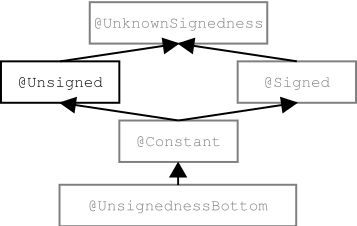
\includegraphics[width=0.4\textwidth]{unsignedness}
    \caption{The type qualifier hierarchy of the Unsignedness annotations.
Qualifiers in gray are used internally by the type system but should never be written by a programmer.}
    \label{fig:my_label}
\end{figure}

The Unsignedness Type System consists of one user defined type, and four internally used types, described in detail below:

\begin{itemize}
  \item The Unsigned type is the only user defined type. This is the only way it can be introduced into a program. This type signifies that a value is unsigned, that it is not to be put into any situation in which Java's default assumption of signed integers may place the program into a bad state.
  \item The Signed type is similarly meant for signed integers, which Java is free to interpret as it pleases. With the exception of logical right shifts, no operator restrictions are placed on Signed values by the Unsignedness Checker.
  \item The Constant type is for values which are known at compile time, and could potentially be signed or unsigned depending on how the programmer intends to use them. Even negative literals may be used as a convenience placeholder for a large positve unsigned integer, so we say a constant value is both signed and unsigned.
  \item The UnknownSignedness type is for values which are either outside of the Unsignedness Checker's scope, or have been mixed so that the Unsignedness Checker no longer knows what signedness to assign to them. In the second case, the presence of an UnknownSignedness value almost always indicates an issue.
  \item The UnsignednessBottom type is never assigned to anything, and if this type is present in an AST, there is an issue.
\end{itemize}

Furthermore, the type system prevents the third class of unsigned integer bugs, the interchange of signed and unsigned integers, by the nature of its hierarchy, shown in Figure~\ref{fig:my_label}.

Types are introduced into a program either by the user, for Unsigned values, or by the the Unsignedness Checker using its type introduction rules. The type introduction rules are best understood through Figure 2, which depicts a flow chart for determining the type of an expression.

% I haven't created the flow chart yet but I think it would be a good way to visually show the introduction rules.

The real work of the Unsignedness Type System is done by its type rules, which eliminate the first two classes of bugs associated with unsigned integers. Generally speaking, these type rules are as follows:

\begin{itemize}
  \item Unsigned values may not be used as input for sensitive operators, as such operators are implemented in Java for signed integers.
  \item With the exception of shifts, no operator may take as input a mix of Signed and Unsigned values.
  \item Logical right shifts may only be applied to Unsigned values.
  \item Arithmetic right shifts may only be applied to Signed values.
\end{itemize}

These rules prevent Unsigned numbers from being used in ways which would allow Java to incorrectly handle them. As ultimately unsigned integers are simply an alternitive representation, we are concerned only that the representation is conserved. This means that the signed implementation of an insensitive operator may be used on an Unsigned value because the result is the same as if the unsigned implementation were used.

\section{Background and Implementation}

% I will go over this section later to include citations. Right now I just want to get words on paper.

We seek here to build a verification tool, so that developers may use it to be sure that their software is free of bugs related to unsigned integers. This means that our approach must be sound; that if it says a program is free of bugs it is so. We build our solution on top of the Checker Framework, an API developed by the University of Washington to provide a platform for pluggable type systems to be introduced into a custom version of the javac compiler. This allows our type system to be checked concurrently with that of Java, and potentially other type systems.

The Checker Framework provides the groundwork for many similar type systems solving other common classes of bugs. Such verification tools, called checkers, provide an excellent template to follow when implementing a type system in this framework. We discussed the Unsignedness Type System, which at a high level consists of a series of qualifiers with some hierarchy, a series of introduction rules for determining expression types, and several type rules for issuing errors for malformed code. These parts are implemented in a checker as follows:

\begin{itemize}
  \item Type qualifiers are implemented with type annotations. The Checker Framework provides several helper annotations to allow the structure of the type hierarchy and some introduction rules to be defined declaratively.
  \item More complex introduction rules are used proceduarally to determine the type of expression trees in the syntax tree using a type factory.
  \item Type rules are enforced by a visitor which visists each node of the syntax tree to determine if it follows type rules.
\end{itemize}

% It would probably be wise here to discuss other checkers and what we can learn from them

\section{Results and Contributions}
% I will go back through this section and cite where needed

To put the Unsignedness Checker to the test, we used it to analyse jake2, a Java port of the popular '90s video game, Quake II. This case study is a large, complex piece of software, with many instances of unsigned integers being used in system code. Without applying annotations the Unsignedness Checker listed many percieved errors with using a logical right shift, sometimes called an unsigned right shift, on signed operands. Many of these were eliminated by annotating documented unsigned integers, but a few persisted. By comparing jake2 with the original C implementation, we have been able to identify and record semanitcal differences between the two systems, particularly in the usage of right shifts. Further analysis is required to determine if these differences have noticiable effects to end users. Furthermore, we have been able to identify one bug, in which an unsigned integer is passed to a utility function which prints its value during debugging. No special handling of the unsigned value is done, so it is printed as if signed, which can possibly lead to erroneous output for values outside signed positive range.

% I will edit this to include examples of the semantic differences and possibly the bug

\bibliographystyle{abbrvnat}

% The bibliography should be embedded for final submission.

\begin{thebibliography}{}
\softraggedright

\bibitem[Smith et~al.(2009)Smith, Jones]{smith02}
P. Q. Smith, and X. Y. Jones. ...reference text...

\end{thebibliography}


\end{document}
